If the weights and the bias are initialized to a random value, the prediction of the perceptron will not be correct. The loss function will measure the distance between the prediction and the ground truth, and the gradient of the loss function will point in the direction of the correct prediction. The weights and the bias will be updated in the direction of the correct prediction, and the prediction will be closer to the ground truth. This process will be repeated until the prediction is correct. This is the perceptron learning algorithm.

\begin{figure}[htbp]
  \centering
  \begin{minipage}{0.45\textwidth}
    \centering
    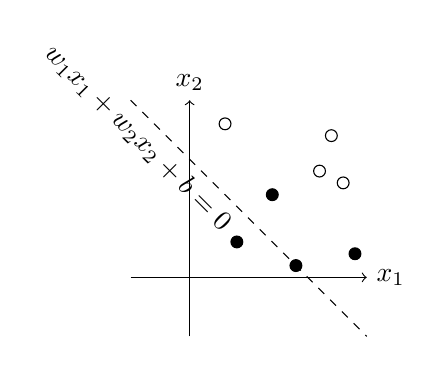
\begin{tikzpicture}[scale=1.5]
        % Positive and negative data points
        \filldraw [black] (0.4,0.3) circle (0.05); %node [below left] {$(1,0)$};
        \filldraw [black] (0.7,0.7) circle (0.05); %node [above] {$(1,1)$};
        \filldraw [black] (0.9,0.1) circle (0.05); %node [below left] {$(1,0)$};
        \filldraw [black] (1.4,0.2) circle (0.05); %node [below right] {$(2,0)$};
        \draw [black] (0.3,1.3) circle (0.05); %node [above left] {$(1,1)$};
        \draw [black] (1.2,1.2) circle (0.05); %node [above right] {$(2,1)$};
        \draw [black] (1.1,0.9) circle (0.05); %node [right] {$(2,1)$};
        \draw [black] (1.3,0.8) circle (0.05); %node [above right] {$(2,1)$};
        
        % Initial decision boundary
        \draw [dashed] (-0.5,1.5) -- (1.5,-0.5) node [midway, below left, sloped] {$w_1x_1 + w_2x_2 + b = 0$};
        
        % Axis labels
        \draw [->] (-0.5,0) -- (1.5,0) node [right] {$x_1$};
        \draw [->] (0,-0.5) -- (0,1.5) node [above] {$x_2$};
    \end{tikzpicture}
    \caption{Bad classification}
  \end{minipage}
  \hfill
  \begin{minipage}{0.45\textwidth}
    \centering
    \begin{tikzpicture}[scale=1.5]
        % Positive and negative data points
        \filldraw [black] (0.4,0.3) circle (0.05); %node [below left] {$(1,0)$};
        \filldraw [black] (0.7,0.7) circle (0.05); %node [above] {$(1,1)$};
        \filldraw [black] (0.9,0.1) circle (0.05); %node [below left] {$(1,0)$};
        \filldraw [black] (1.4,0.2) circle (0.05); %node [below right] {$(2,0)$};
        \draw [black] (0.3,1.3) circle (0.05); %node [above left] {$(1,1)$};
        \draw [black] (1.2,1.2) circle (0.05); %node [above right] {$(2,1)$};
        \draw [black] (1.1,0.9) circle (0.05); %node [right] {$(2,1)$};
        \draw [black] (1.3,0.8) circle (0.05); %node [above right] {$(2,1)$};

        % Initial decision boundary
        \draw [dashed] (-0.5,1.5) -- (1.5,0.5) node [midway, below left, sloped] {$w_1x_1 + w_2x_2 + b = 0$};
        
        % Axis labels
        \draw [->] (-0.5,0) -- (1.5,0) node [right] {$x_1$};
        \draw [->] (0,-0.5) -- (0,1.5) node [above] {$x_2$};
    \end{tikzpicture}
    \caption{Good classsification}
  \end{minipage}
\end{figure}
